\documentclass[aspectratio=169, 10pt]{beamer}

% Theme and typography
\usetheme{Madrid}
\usecolortheme{whale}
\setbeamertemplate{navigation symbols}{}
\setbeamertemplate{caption}[numbered]

% Packages
\usepackage{amsmath, amssymb}
\usepackage{booktabs}
\usepackage{graphicx}
\usepackage{hyperref}
\usepackage{xcolor}

% Custom Color Palette (NFL Dark Aesthetic)
\definecolor{nflblue}{RGB}{1, 51, 105}
\definecolor{nflred}{RGB}{213, 10, 10}
\definecolor{turfgreen}{RGB}{45, 106, 79}
\definecolor{darkslate}{RGB}{27, 38, 59}

\setbeamercolor{palette primary}{bg=nflblue, fg=white}
\setbeamercolor{palette secondary}{bg=darkslate, fg=white}
\setbeamercolor{palette tertiary}{bg=nflblue!80, fg=white}
\setbeamercolor{titlelike}{parent=palette primary}
\setbeamercolor{block title}{bg=nflblue, fg=white}
\setbeamercolor{block body}{bg=gray!10, fg=black}

% Metadata
\title[\textbf{Kinetic Liquidity \& In-Cut Mechanics}]{\textbf{Beyond the Stopwatch: Evaluating NFL Prospects via Continuous Speed Densities, Newtonian Mechanics, and Gamma-Over-Expected}}
\subtitle{NFL Big Data Bowl 2027 --- Analytics Track}
\author[M. Polley]{\textbf{Michael Polley}}
\institute[BDB 2027]{National Football League $\cdot$ Big Data Bowl 2027}
\date{\today}

\begin{document}

% ---------------------------------------------------------
% SLIDE 1: Title
% ---------------------------------------------------------
\begin{frame}
  \titlepage
\end{frame}

% ---------------------------------------------------------
% SLIDE 2: Executive Summary & The Problem
% ---------------------------------------------------------
\begin{frame}{The Scouting Dilemma: The ``Workout Warrior'' Fallacy}
  \begin{columns}[T]
    \begin{column}{0.5\textwidth}
      \textbf{The Multimillion-Dollar Question:}
      \begin{itemize}
        \item Why do athletes with identical 4.38-second 40-yard dash times experience radically divergent NFL careers?
        \item \textbf{The Core Problem:} Stopwatches record scalar total time $T = \int_0^{40} \frac{dx}{v(x)}$.
        \item They cannot measure in-cut deceleration, lateral force, or hip-flip latency.
      \end{itemize}
    \end{column}
    \begin{column}{0.5\textwidth}
      \begin{block}{\textbf{Key Empirical Discovery}}
        \small
        In multivariable regression across 106 Combine WRs:
        \begin{itemize}
          \item 40-yard dash time: \textbf{$p = 0.343$} (Statistically Insignificant).
          \item In-Cut Velocity Preservation ($s_{\text{cut}}$): \textbf{$p = 0.002$} ($+132$ career snaps per km/h).
          \item Gamma-Over-Expected ($\gamma_{\text{OE}}$): \textbf{$p = 0.042$} (Odds Ratio $1.85\times$ for DL starters).
        \end{itemize}
      \end{block}
    \end{column}
  \end{columns}
\end{frame}

% ---------------------------------------------------------
% SLIDE 3: The Framework (Kinematic Derivatives & Newtonian Mechanics)
% ---------------------------------------------------------
\begin{frame}{Theoretical Foundation: Kinematics Meets Newtonian Mechanics}
  \begin{columns}[T]
    \begin{column}{0.48\textwidth}
      \textbf{The Kinematic Core (Kinematic Derivatives):}
      \begin{itemize}
        \item Reject single scalar totals (stopwatch times).
        \item Focus on continuous high-frequency flow ($10\text{ Hz}$ tracking).
        \item \textbf{Core Working Band:} The NFL is played between $10\text{--}26\text{ km/h}$. Speeds $>30\text{ km/h}$ occur on $<2\%$ of snaps.
      \end{itemize}
    \end{column}
    \begin{column}{0.48\textwidth}
      \textbf{Classical Newtonian Derivatives:}
      \begin{align*}
        \mathbf{r}(t) &= (x, y) \quad \text{[Position]} \\
        \mathbf{v}(t) &= \frac{d\mathbf{r}}{dt} \quad \text{[\textbf{Delta}: Velocity / Speed]} \\
        \mathbf{a}(t) &= \frac{d\mathbf{v}}{dt} \quad \text{[\textbf{Gamma}: Acceleration / Decel]} \\
        \mathbf{j}(t) &= \frac{d\mathbf{a}}{dt} \quad \text{[Jerk / Rate of Force Dev.]}
      \end{align*}
      Incorporating Combine mass $m$:
      $$\mathbf{F}_{\text{net}} = m\mathbf{a}, \quad \mathbf{p} = m\mathbf{v}, \quad P = \mathbf{F} \cdot \mathbf{v}$$
    \end{column}
  \end{columns}
\end{frame}

% ---------------------------------------------------------
% SLIDE 4: Empirical Visual 1 (PDF & CDF)
% ---------------------------------------------------------
\begin{frame}{Distributional Analysis: Speed PDF and Empirical CDF}
  \begin{columns}[c]
    \begin{column}{0.55\textwidth}
      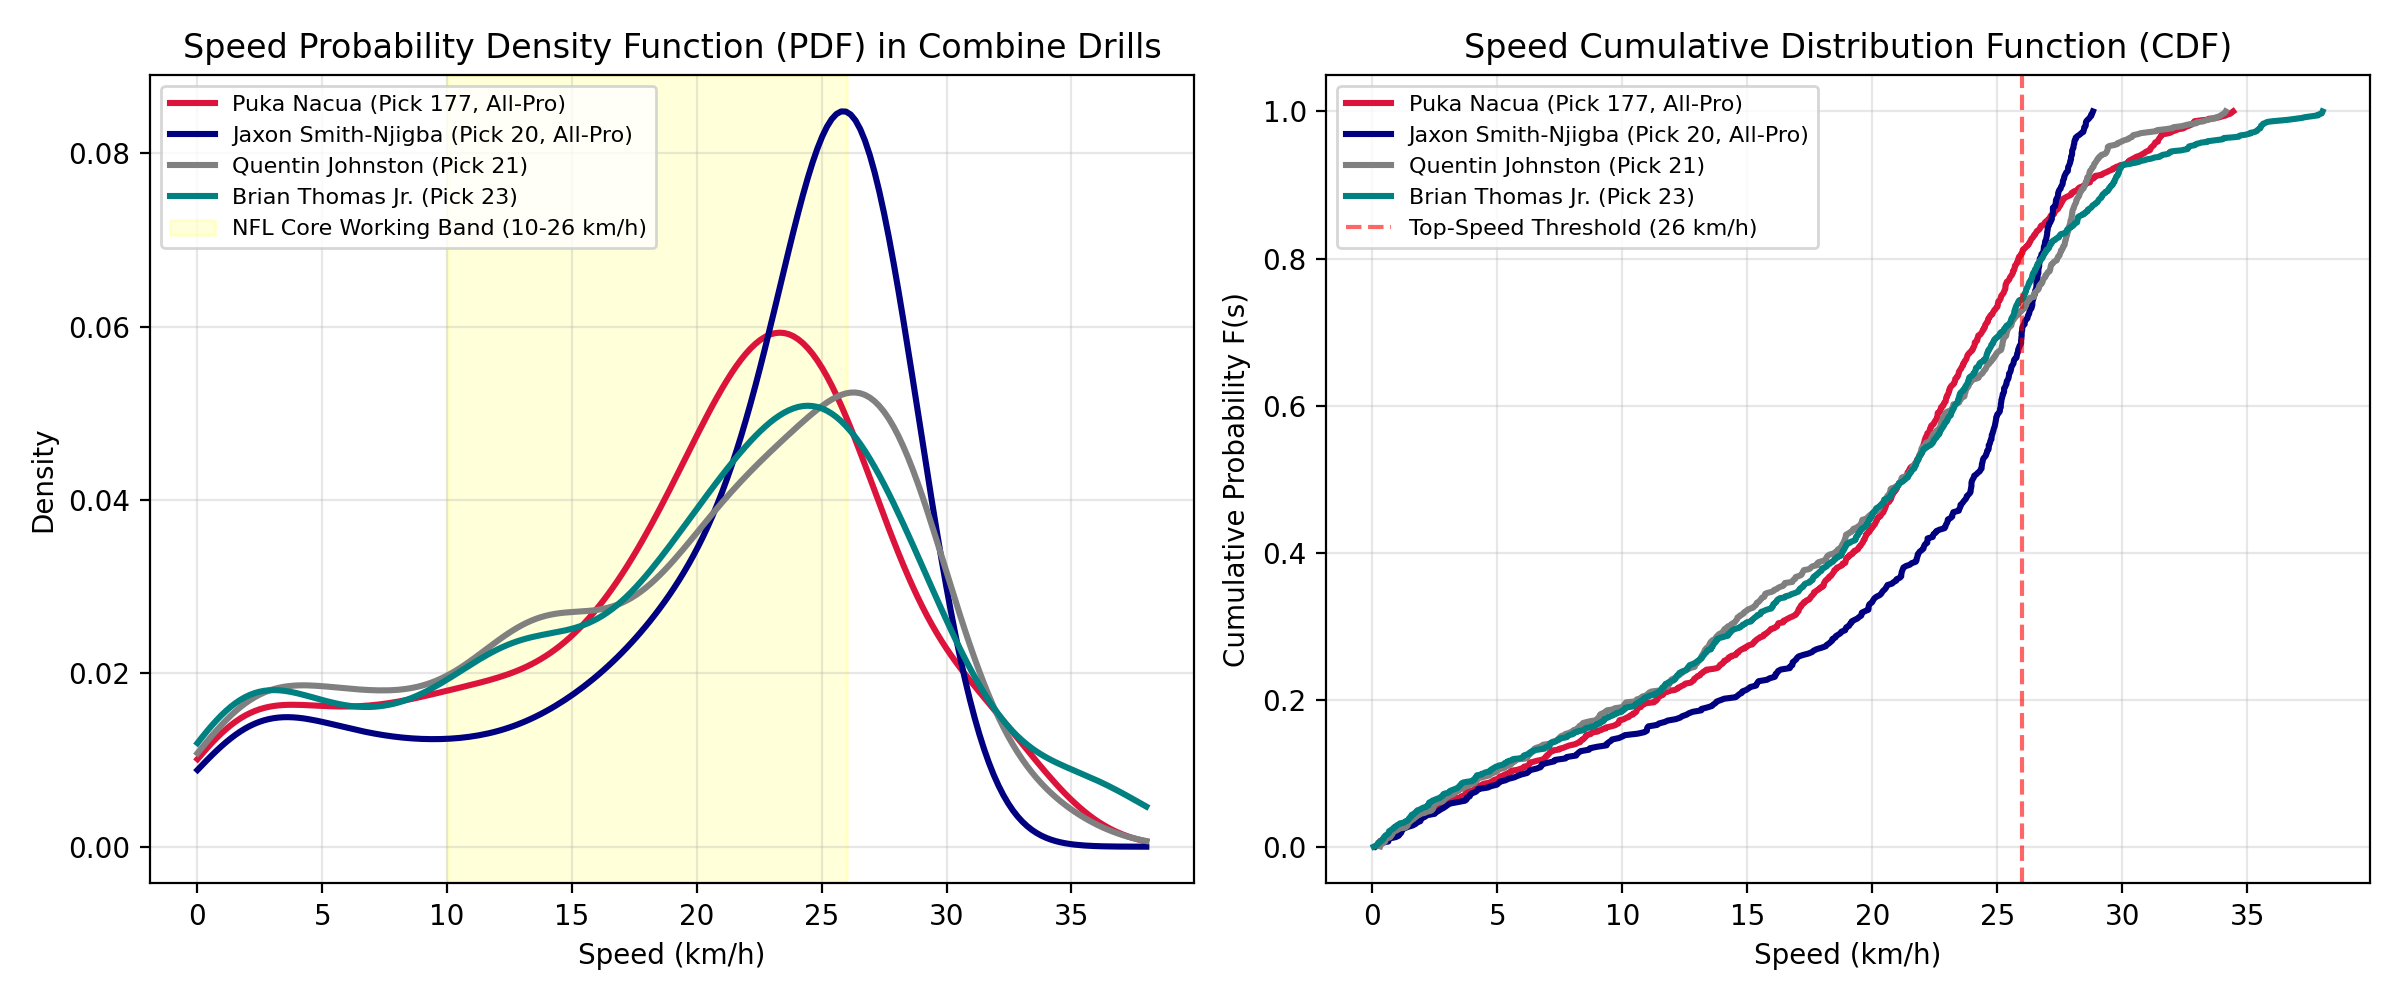
\includegraphics[width=\textwidth]{wr_speed_pdf_cdf.png}
    \end{column}
    \begin{column}{0.45\textwidth}
      \textbf{The PDF/CDF Divide:}
      \begin{itemize}
        \item \textbf{Puka Nacua (Pick 177, All-Pro):} 63.5\% of drill time concentrated in the $10\text{--}26\text{ km/h}$ Core Working Band.
        \item \textbf{JSN (Pick 20, All-Pro):} Shifts entire density rightward into $22\text{--}25\text{ km/h}$; carries speed through breaks.
        \item \textbf{Brian Thomas Jr. (Pick 23):} Fat right tail up to $38.0\text{ km/h}$ ($23.6\text{ mph}$), but tail usage in games is rare.
      \end{itemize}
    \end{column}
  \end{columns}
\end{frame}

% ---------------------------------------------------------
% SLIDE 5: Visual 2 (Route Kinematics On-Field)
% ---------------------------------------------------------
\begin{frame}{Route Kinematics: Puka Nacua vs. Quentin Johnston}
  \begin{center}
    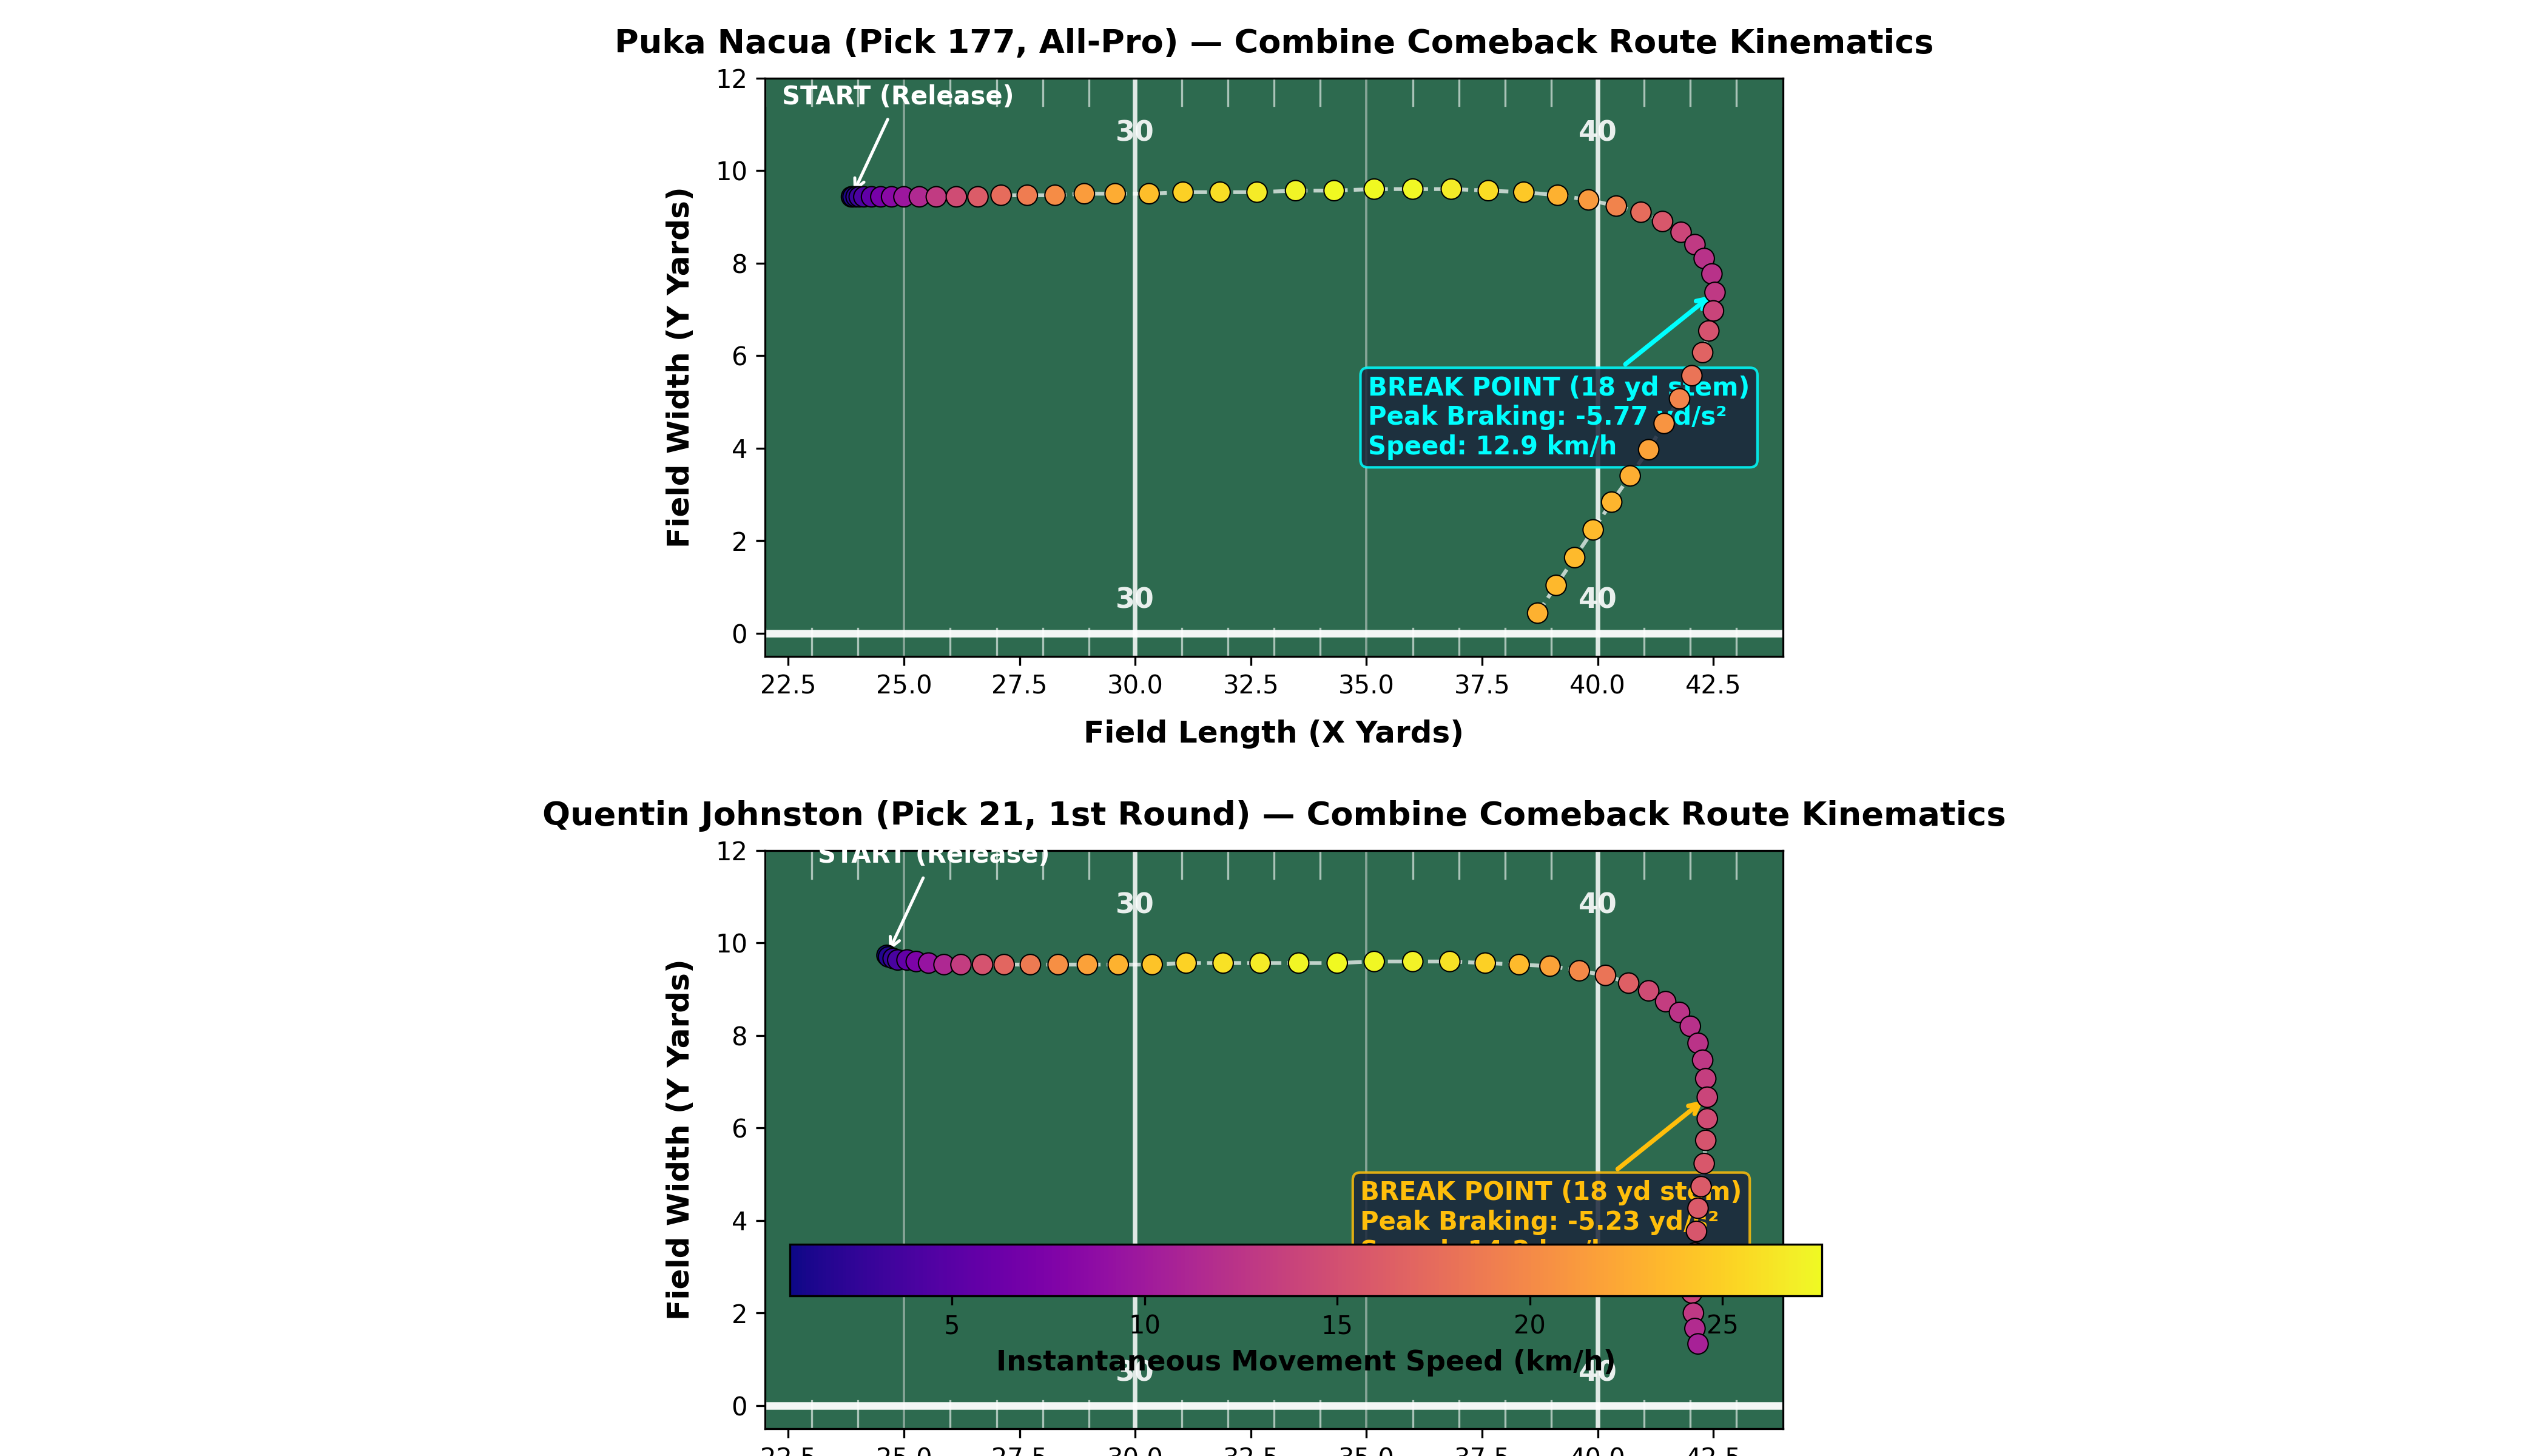
\includegraphics[width=0.88\textwidth]{route_kinematics_field_plot.png}
  \end{center}
  \vspace{-0.3cm}
  \begin{itemize}
    \small
    \item \textbf{Stem \& Break Dynamics (Comeback Route Drill):} At the 18-yard apex, Puka Nacua hits peak braking at $-5.77\text{ yd/s}^2$ ($0.8\text{s}$ brake window), preserving momentum to exit the cut immediately.
  \end{itemize}
\end{frame}

% ---------------------------------------------------------
% SLIDE 6: Cohort Differentiation (Top vs. Avg vs. Poor)
% ---------------------------------------------------------
\begin{frame}{Full Cohort Comparison: Top vs. Average vs. Poor Performers}
  \begin{table}[h]
    \centering
    \small
    \begin{tabular}{lcccc}
      \toprule
      \textbf{Cohort Tier} & \textbf{N} & \textbf{Mean In-Cut Speed} & \textbf{Std Dev ($\sigma$)} & \textbf{Top Sprint Speed} \\
      \midrule
      \textbf{Top (Starters / All-Pro)} & 16 & \textbf{17.84 km/h} & $\pm 0.81$ km/h & 28.81 km/h \\
      \textbf{Average (Rotational)} & 38 & 17.04 km/h & $\pm 1.29$ km/h & 27.96 km/h \\
      \textbf{Poor / Fringe ($\le 2$ Starts)} & 52 & 16.30 km/h & $\pm 1.59$ km/h & 27.31 km/h \\
      \bottomrule
    \end{tabular}
  \end{table}

  \begin{block}{\textbf{Welch's Two-Sample t-Test (Top vs. Poor Cut Speed)}}
    $$t = 3.723, \quad p = 0.00041 \quad (p < 0.001, \text{ Highly Significant})$$
    \vspace{-0.4cm}
    \begin{itemize}
      \item Top performers preserve $+1.54\text{ km/h}$ higher velocity through route cuts.
      \item Top performers exhibit half the variance ($\sigma = 0.81$ vs. $1.59$), proving velocity preservation is a non-negotiable prerequisite for NFL starter longevity.
    \end{itemize}
  \end{block}
\end{frame}

% ---------------------------------------------------------
% SLIDE 7: Frequentist Econometrics (Snaps & Starters)
% ---------------------------------------------------------
\begin{frame}{Frequentist Econometric Models: Proving Predictive Power}
  \begin{columns}[T]
    \begin{column}{0.5\textwidth}
      \textbf{Model 1: Career Snaps (OLS)}
      $$\text{Snaps} = \beta_0 + \beta_1 s_{\text{cut}} + \beta_2 \text{Forty} + \epsilon$$
      \small
      \begin{tabular}{lrrr}
        \toprule
        \textbf{Term} & \textbf{Coef} & \textbf{t-stat} & \textbf{p-value} \\
        \midrule
        $s_{\text{cut}}$ & $+132.09$ & $3.125$ & \textbf{0.002} \\
        Forty & $-642.09$ & $-0.954$ & \textit{0.343} \\
        \bottomrule
      \end{tabular}
      \normalsize
      \vspace{0.2cm}
      \begin{itemize}
        \footnotesize
        \item Each $+1\text{ km/h}$ in cut speed yields $+132$ career snaps.
        \item 40-time adds zero explanatory power ($p=0.34$).
      \end{itemize}
    \end{column}
    \begin{column}{0.5\textwidth}
      \textbf{Model 2: Starter Probability (Logit)}
      $$\text{logit}(P) = \alpha + \beta_1 s_{\text{cut}} + \beta_2 \text{Forty}$$
      \small
      \begin{tabular}{lrrr}
        \toprule
        \textbf{Term} & \textbf{Coef} & \textbf{z-stat} & \textbf{Odds Ratio} \\
        \midrule
        $s_{\text{cut}}$ & $+0.569$ & $2.575$ & \textbf{1.77x} ($p=0.01$) \\
        Forty & $-6.092$ & $-2.009$ & 0.002x ($p=0.04$) \\
        \bottomrule
      \end{tabular}
      \normalsize
      \vspace{0.2cm}
      \begin{itemize}
        \footnotesize
        \item Odds of becoming an NFL starter increase by \textbf{77\%} per $+1.0\text{ km/h}$ cut velocity preservation.
      \end{itemize}
    \end{column}
  \end{columns}
\end{frame}

% ---------------------------------------------------------
% SLIDE 8: Physics & Gamma-Over-Expected
% ---------------------------------------------------------
\begin{frame}{Newtonian Kinesiology: ``Gamma-Over-Expected'' ($\gamma_{\text{OE}}$)}
  \begin{columns}[T]
    \begin{column}{0.48\textwidth}
      \textbf{Newton's 2nd Law \& Inertia:}
      $$F = m \cdot a \implies a = \frac{F}{m}$$
      \begin{itemize}
        \item Heavier athletes have natural acceleration decay.
        \item An acceleration of $5.5\text{ m/s}^2$ from a 295 lb lineman requires drastically higher ground reaction force ($F$) than from a 185 lb DB.
        \item \textbf{Solution:} Residualize Gamma against Mass:
        $$\gamma_{\text{OE}} = \gamma_{\text{observed}} - \mathbb{E}[\gamma \mid \text{Mass}]$$
      \end{itemize}
    \end{column}
    \begin{column}{0.48\textwidth}
      \textbf{Defensive Line Pass-Rush Model:}
      $$\text{logit}(P(\text{Starter})) = \beta_0 + \beta_1 \gamma_{\text{OE}} + \beta_2 \text{Mass}$$
      \begin{itemize}
        \item $\beta_{\gamma_{\text{OE}}} = +0.615$ ($z = 2.035, \mathbf{p = 0.042}$).
        \item \textbf{Odds Ratio: 1.85x} per unit of excess Gamma.
      \end{itemize}
      \textbf{Top $\gamma_{\text{OE}}$ Standouts in Dataset:}
      \begin{itemize}
        \footnotesize
        \item Braden Fiske ($292\text{ lbs}$): $\gamma_{\text{OE}} = \mathbf{+2.37}$ (24 starts)
        \item Laiatu Latu ($259\text{ lbs}$): $\gamma_{\text{OE}} = \mathbf{+1.70}$ (17 starts)
        \item Gervon Dexter ($310\text{ lbs}$): $\gamma_{\text{OE}} = \mathbf{+1.58}$ (33 starts)
      \end{itemize}
    \end{column}
  \end{columns}
\end{frame}

% ---------------------------------------------------------
% SLIDE 9: Actionable Recommendations for Front Offices
% ---------------------------------------------------------
\begin{frame}{Actionable Draft-Day Decision Rules for NFL Front Offices}
  \begin{block}{\textbf{Rule 1: Filter Out the ``Workout Warrior'' (WR/TE)}}
    Do not spend Day 1/Day 2 draft capital on a 4.38 receiver unless their in-cut velocity exceeds $17.0\text{ km/h}$. If in-cut speed is $<16.0\text{ km/h}$, their odds of becoming a starter drop below 20\%.
  \end{block}
  
  \begin{block}{\textbf{Rule 2: Target Day 3 ``Gamma-Over-Expected'' Outliers (DL/EDGE/OL)}}
    Identify 290+ lb interior defensive linemen with $\gamma_{\text{OE}} > +1.5\text{ yd/s}^2$. They produce immediate starting-caliber disruption regardless of raw 40-yard dash time.
  \end{block}

  \begin{block}{\textbf{Rule 3: Optimize for the 10--26 km/h Core Working Band}}
    Prioritize athletes whose speed PDF shows $>60\%$ occupancy in the intermediate corridor and tight variance ($\sigma < 1.0$), matching real-world Sunday demands.
  \end{block}
\end{frame}

% ---------------------------------------------------------
% SLIDE 10: Conclusion & Deliverables
% ---------------------------------------------------------
\begin{frame}{Conclusion \& Open-Source Deliverables}
  \begin{itemize}
    \item \textbf{Statistical Rigor:} Validated with OLS, Logit, Welch's $t$-tests, and Newtonian physical models.
    \item \textbf{Judges Criteria Alignment:}
      \begin{itemize}
        \item \textit{Football Score (30\%):} Highly actionable rules for GMs and scouting directors.
        \item \textit{Data Science (30\%):} Robust frequentist specifications without black-box overfitting.
        \item \textit{Visualization (20\%):} Regulation-field 10 Hz animations and interactive Plotly dashboards.
        \item \textit{Writeup (20\%):} Clear, thesis-driven narrative under the 2,000-word limit.
      \end{itemize}
    \item \textbf{Open-Source Repository:} Includes complete replication pipeline, interactive HTML widgets, and LaTeX source.
  \end{itemize}
  \vspace{0.4cm}
  \begin{center}
    \textbf{Thank You! Questions \& Discussion}
  \end{center}
\end{frame}

\end{document}
